% !TeX encoding = UTF-8
% !TeX spellcheck = russian-aot
% !TeX program = pdflatex
\documentclass[aps,pre,reprint]{revtex4-2}

\usepackage[T2A]{fontenc}
\usepackage[utf8]{inputenc}
\usepackage[russian]{babel}

\usepackage{graphicx}
\usepackage{float}



\begin{document}
	
	\title{Речь к презентации о сортировках слиянием}
	
	\author{В.\,С.\,Верхотуров}
	\altaffiliation{РТУ МИРЭА}
	\email[Электропочта:]{valery.verkhoturov1505@gmail.com}

	\maketitle
	
	\section{Содержание}
	
	\tableofcontents
	
	\section{Слайд~3}
	\begin{figure}[H]
		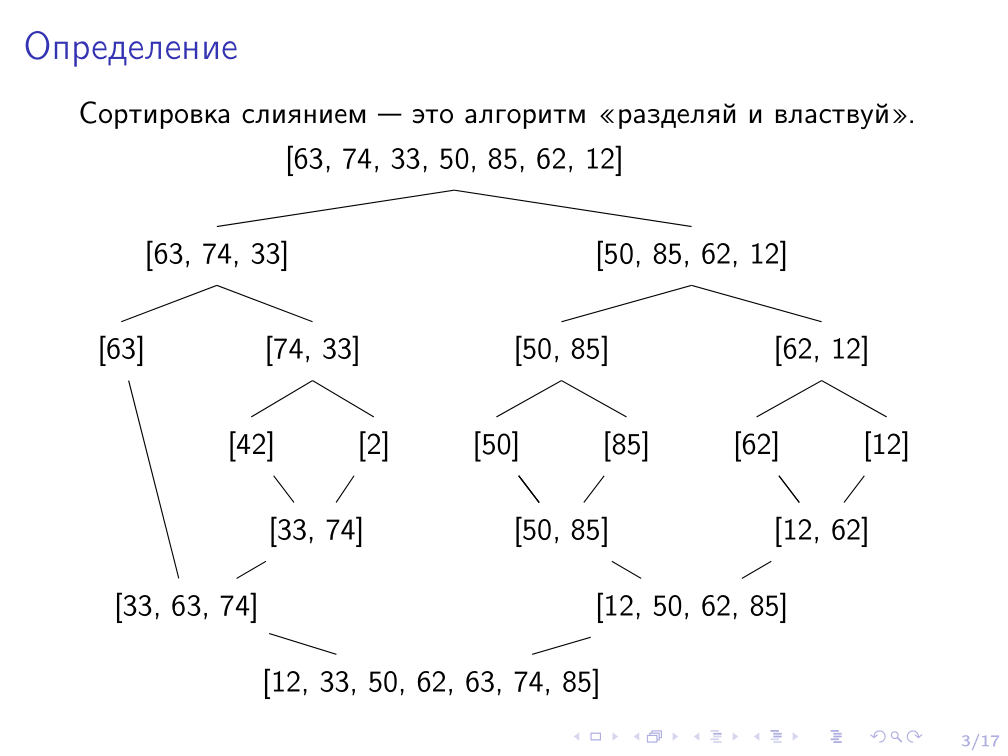
\includegraphics[scale=.6]{presentation-03.png}
	\end{figure}

	
	Сортировка слиянием~--- это алгоритм <<разделяй и властвуй>>. 
	\begin{enumerate}
		\item Он последовательно делит входной список длины n пополам, пока не останется n списков размера 1 (верхняя часть графа);
		\item Затем пары списков объединяются вместе с меньшим первым элементом среди пары списков, добавляемых на каждом шаге (нижняя часть графа).
	\end{enumerate}

	\section{Слайды~4,~5}
	\begin{figure}[H]
		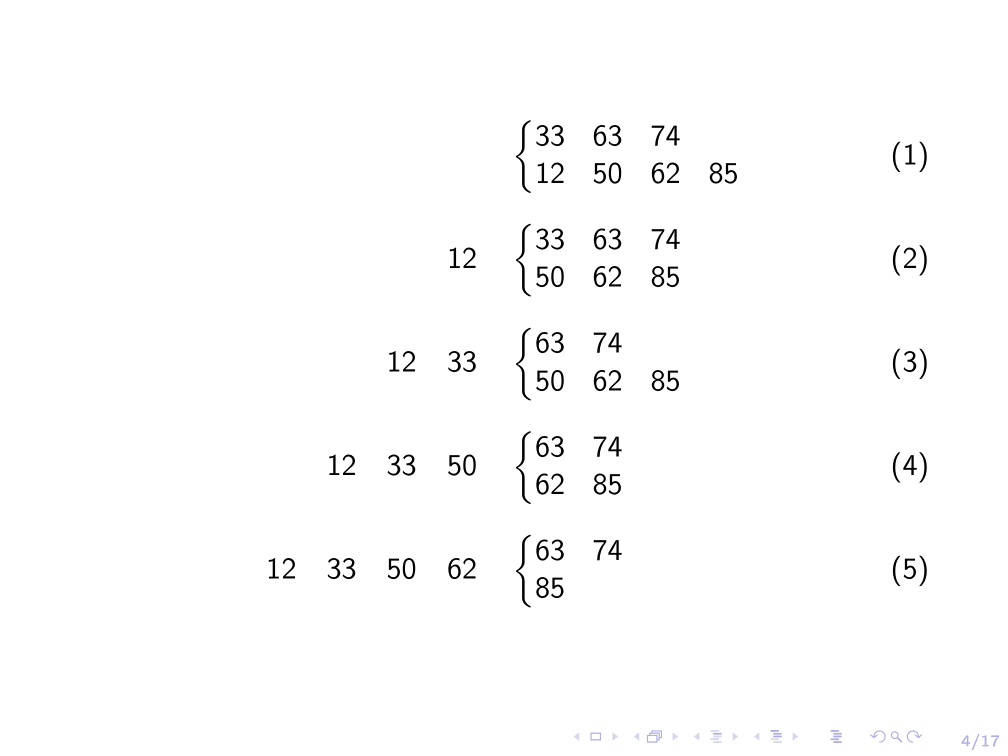
\includegraphics[scale=.7]{presentation-04.png}
		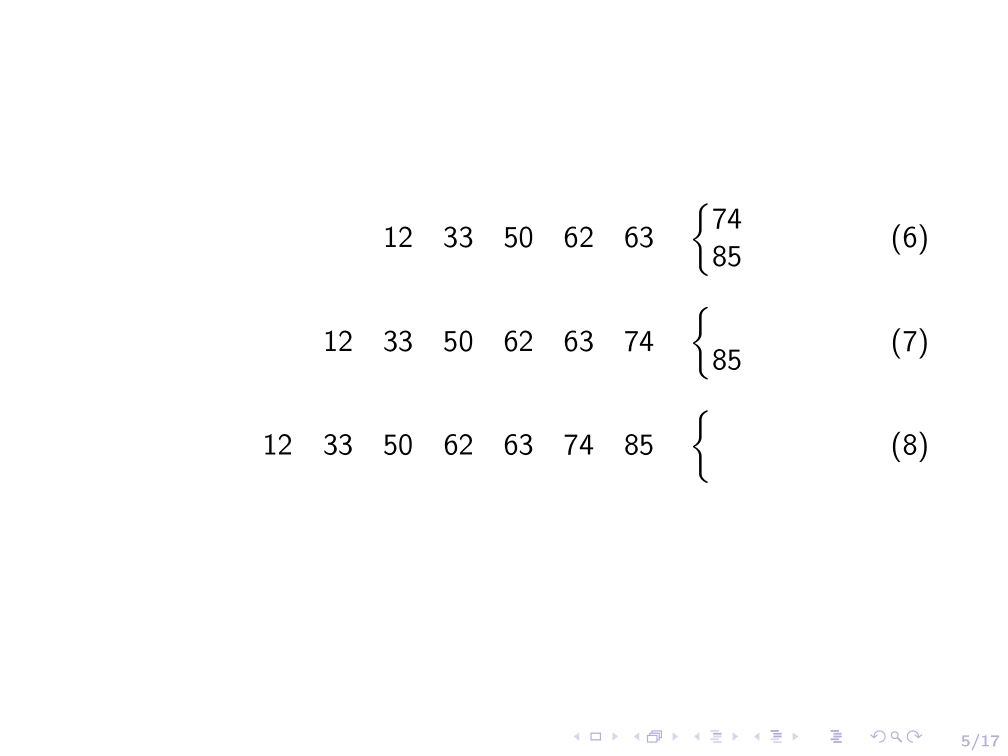
\includegraphics[scale=.7]{presentation-05.png}
	\end{figure}
	
	Принцип объединения списков (merge).
	
	\begin{enumerate}
		\item Даны два массива. Гарантируется, что каждый из массивов отсортирован;
		\item На каждой итерации 1--8 сравниваются первые элементы массива. Наименьший элемент достаётся из исходного массива и добавляется в конец отсортированного массива. Итерации заканчиваются, когда все элементы перешли в отсортированный массив.
	\end{enumerate}

	\section{Слайд~6}
	\begin{figure}[H]
		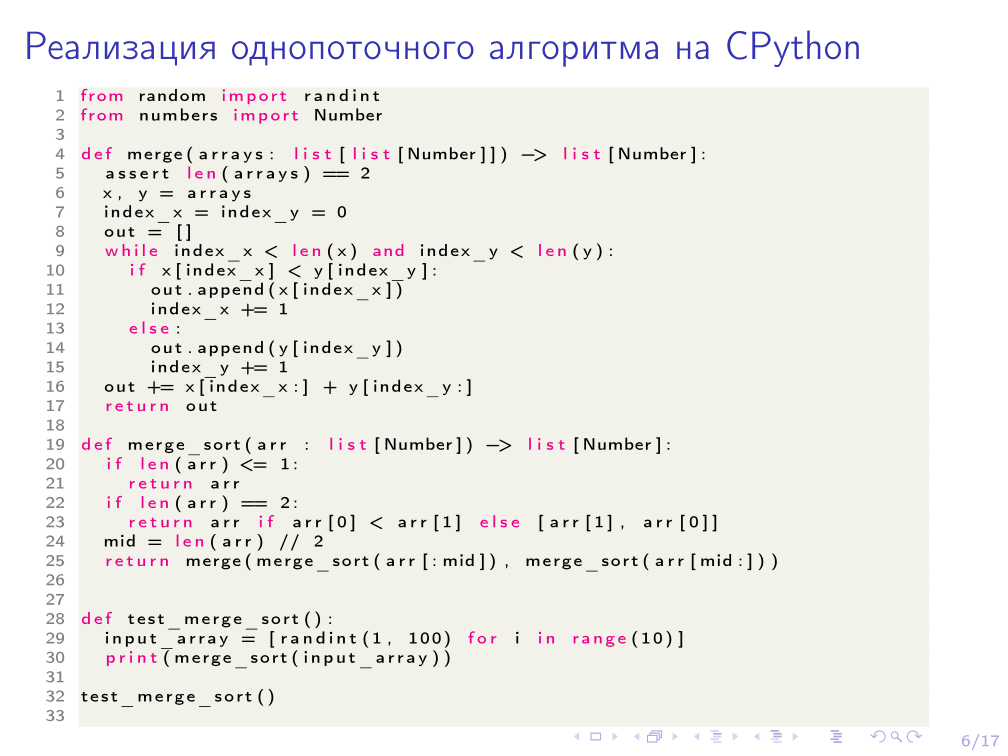
\includegraphics[scale=.7]{presentation-06.png}
	\end{figure}
	
	Код на Python читается снизу вверх. Разобран на слайдах 7, 8, 9.
	
	\section{Слайд~7}
	\begin{figure}[H]
		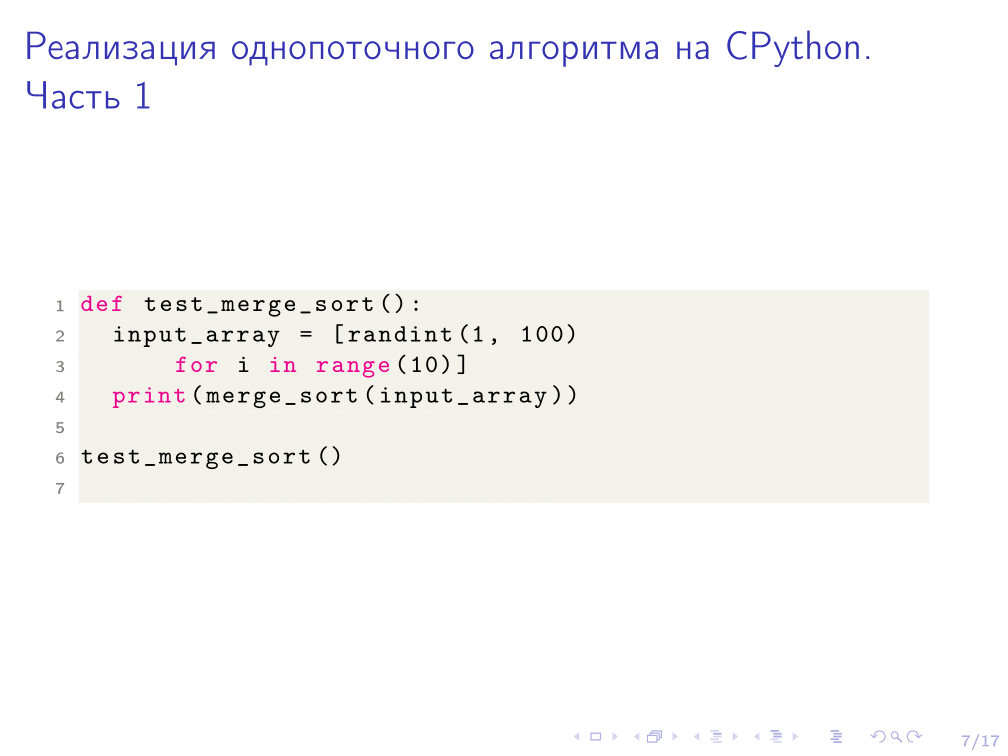
\includegraphics[scale=.7]{presentation-07.png}
	\end{figure}
	
	\begin{description}
		\item[Строка 1] Определение функции, проверяющей работоспособность алгоритма;
		\item[2, 3] Создание массива из 10 элементов псевдослучайных чисел от 1 до 100;
		\item[4] Сортировка, вывод отсортированного массива;
		\item[6] Вызов функции, определённой в строке 1, проверяющей работоспособность алгоритма.
	\end{description}

	\section{Слайд~8}
	\begin{figure}[H]
		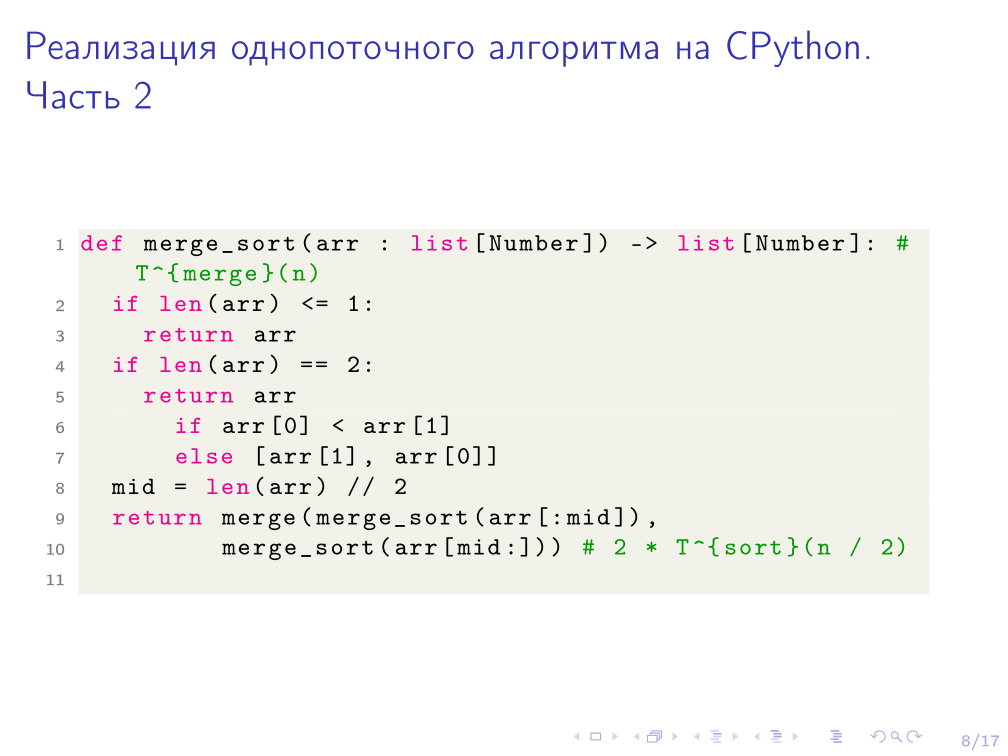
\includegraphics[scale=.7]{presentation-08.png}
	\end{figure}
	
	\begin{description}
		\item[1] Определении функции, которая разделяет исходный массив пополам в рекурсии, сливает и возвращает;
		\item[2--3] Если длинна массива равна 0 или 1, то массив возвращается без изменений;
		\item[4--7] Массив из 2 элементов сортируется. Если первый элемент меньше второго, то возвращается без изменений, иначе элементы меняются местами, изменённый массив возвращается;
		\item[8, 9] Если массив состоит больше, чем из двух элементов, то находится индекс посередине массива, массив делится на две половины \verb*|arr[:mid]| и \verb*|arr[mid:]|, каждая половина рекурсивно сортируется $T^{sort}(n \times 2)$, вместе сливаются $2 \times T^{sort}(n \times \times 2)$.
	\end{description}

	\section{Слайд~9}
	\begin{figure}[H]
		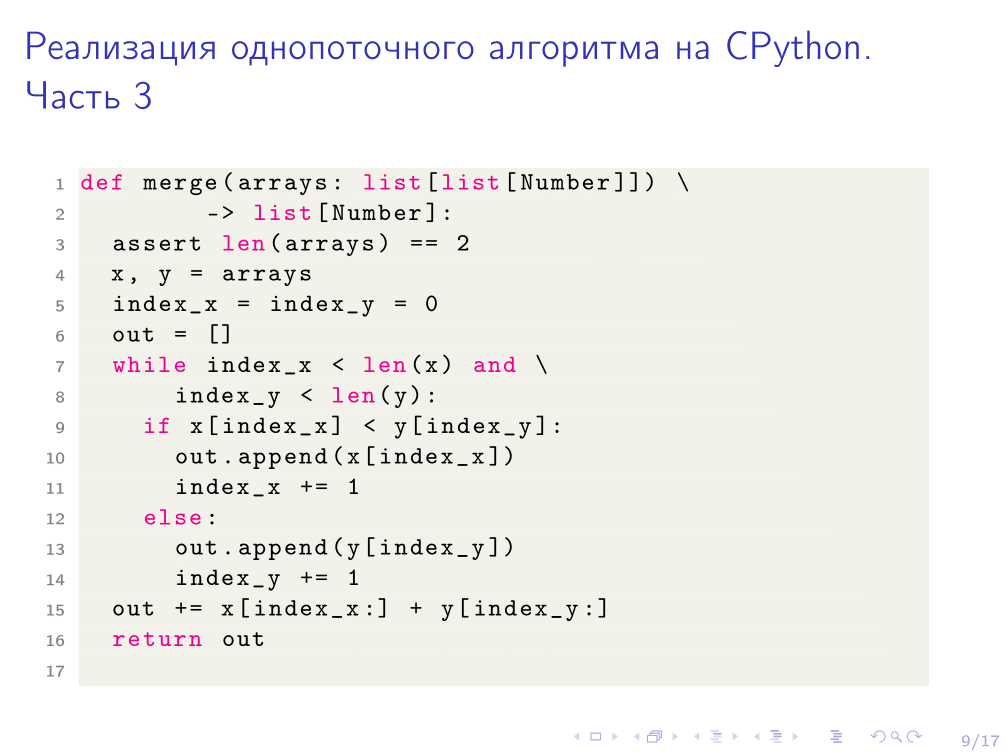
\includegraphics[scale=.7]{presentation-09.png}
	\end{figure}
	
	\begin{description}
		\item[1, 2] Определении функции слияния, которая принимает массив с двумя сортированными массивами и возвращает один отсортированный массив;
		\item[3] Проверка, находятся ли в принимаемом массиве два внутренних массива,
		\item[4] $x$~--- первый внутренний массив, $y$~--- второй внутренний массив;
		\item[5] Индексы первых элементов массивов $x$, $y$, которые будут сравниваться, равны 0;
		\item[6] Создание пустого выходного массива;
		\item[7--8] Пока в массиве $x$ И $y$ есть хотя бы по одному элементу, то:
		\begin{description}
			\item[9-14] Добавить в выходной массив наименьшее значение из первых элементов массивов $x$, $y$, увеличить индекс начально элемента того массива, из которого было взято значение;
		\end{description}
		\item[15] Добавить оставшийся элемент к выходному массиву;
		\item[16] Вернуть из функции выходной массив.
	\end{description}

	\textit{Примечание:} на слайдах 4, 5 говорилось об извлечении элемента из исходного, что потребовало бы создание нового массива размера $n - 1$ и копирование элементов исходного массива. Эффективнее увеличить индекс на 1 и принимать его за индекс первого элемента на следующей итерации.
	
	\section{Слайд~10}
	\begin{figure}[H]
		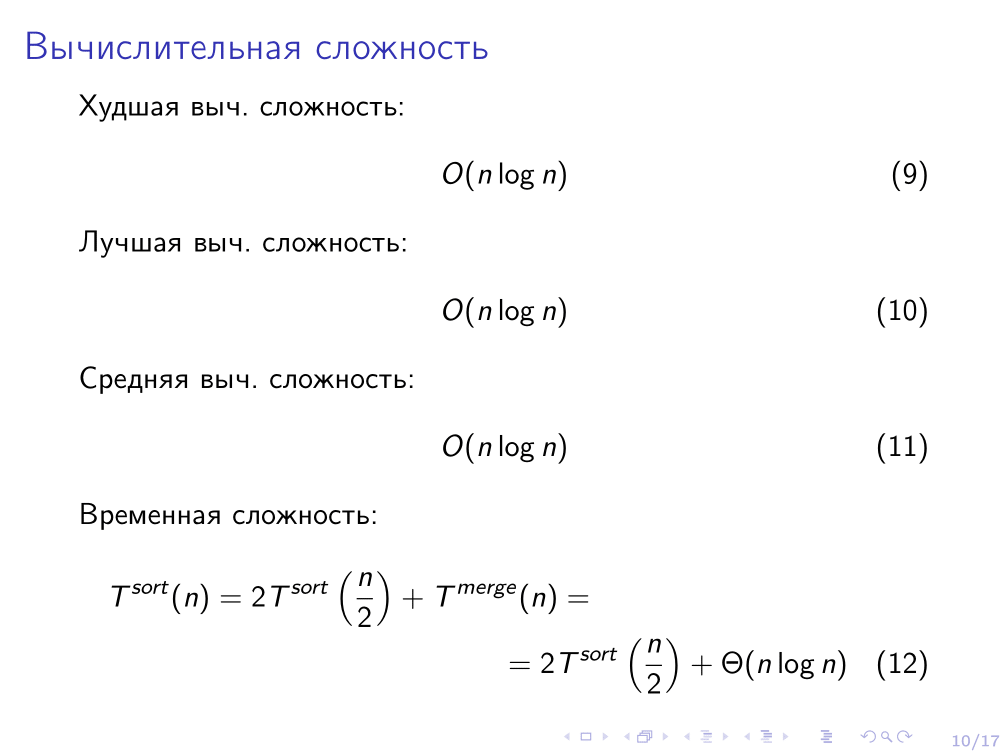
\includegraphics[scale=.7]{presentation-10.png}
	\end{figure}
	
	\section{Слайд~11}
	\begin{figure}[H]
		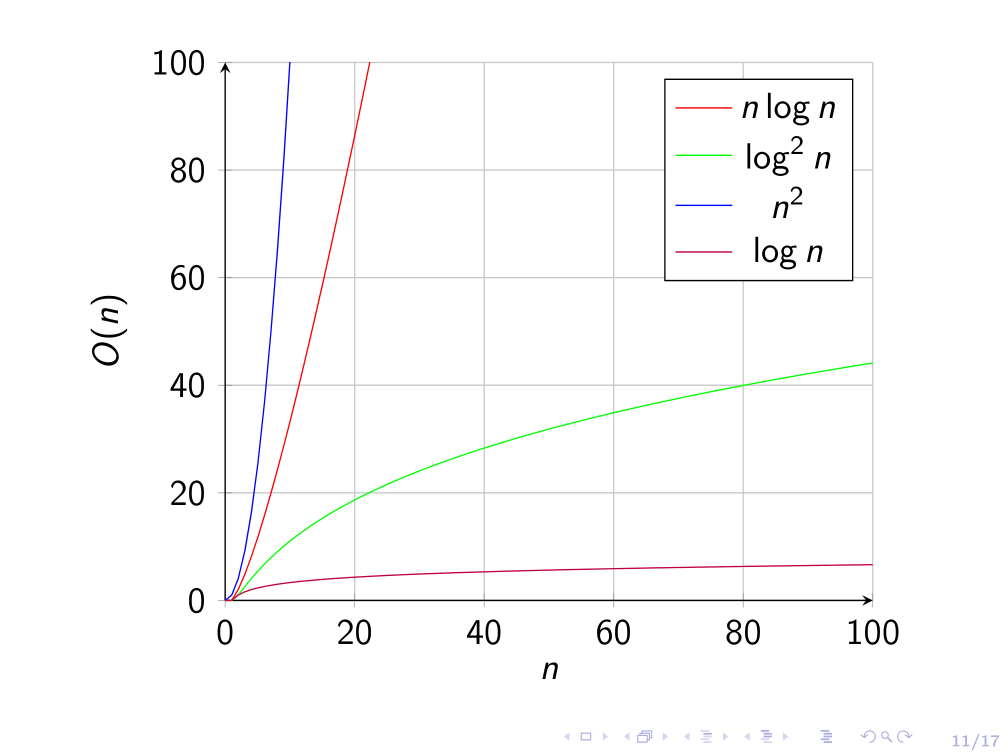
\includegraphics[scale=.7]{presentation-11.png}
	\end{figure}
	
	Средние выч. сложности:
	\begin{description}
		\item[$n\log n$] Выч. сложность однопоточного алгоритма сортировки слиянием;
		\item[$\log^2{}{n}$] Cортировка Бетчера (Bitonic sorter);
		\item[$n^2$] Сортировка пузырьком;
		\item[$\log n$] Параллельная сортировка слиянием.
	\end{description}

	\section{Слайд~12}
	\begin{figure}[H]
		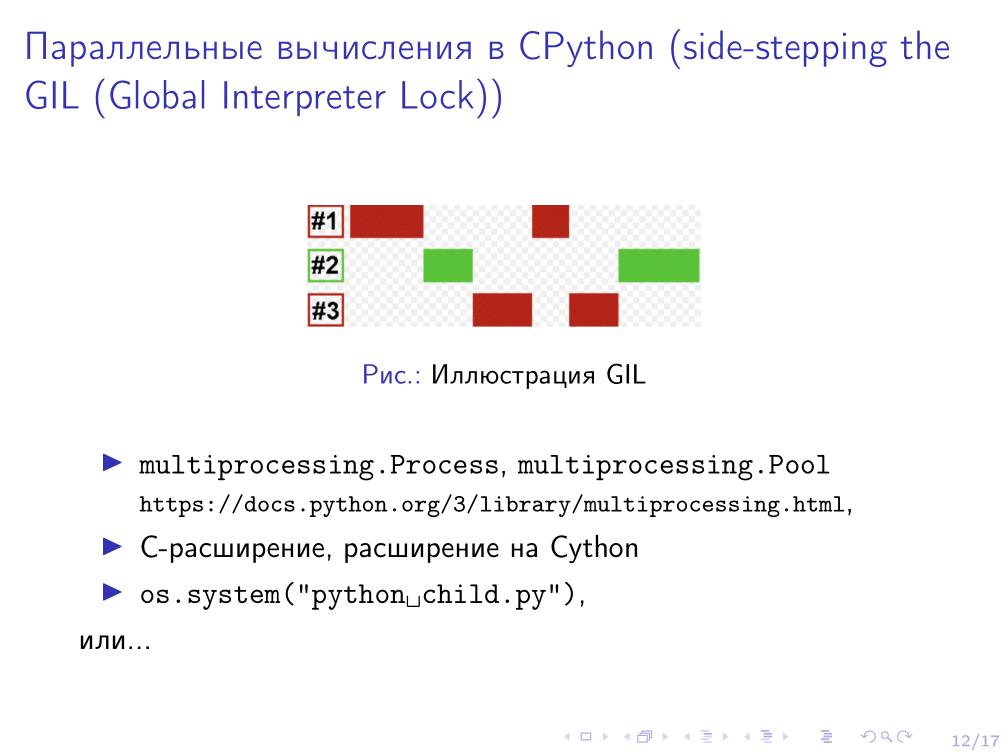
\includegraphics[scale=.7]{presentation-12.png}
	\end{figure}
	
	Наиболее известная реализация Python является CPython (интерпретатор), которая имеет глобальную блокировку интерпретатора, не позволяю распараллелить программу. Асинхронные функции, инструменты стандартных библиотек \verb*|threadig|, \verb*|concurrency| работают конкурентно. Необходимы инструменты, которые обходят блокировщик (side-stepping the GIL):
	\begin{description}
		\item[стандартная библиотека multiprocessing] позволяет разделить задачи по процессам (Process создаёт 1 процесс, Pool~--- много);
		\item[С-расширение] распараллеливание кода на Си, вызванного из CPython;
		\item[Cython] Реализация Python, имеющая возможность обхода блокировщика, возможно написание расширение для CPython;
		\item[Консольная команда] Запуск подпроцесса с помощью консольной команды.
	\end{description}

	\textit{Примечание:} стандартная библиотека \verb*|subprocess| также предоставляет возможность создания подпроцесса c другой программой, не подходит для конкретной задачи.

	\section{Слайд~13}
	\begin{figure}[H]
		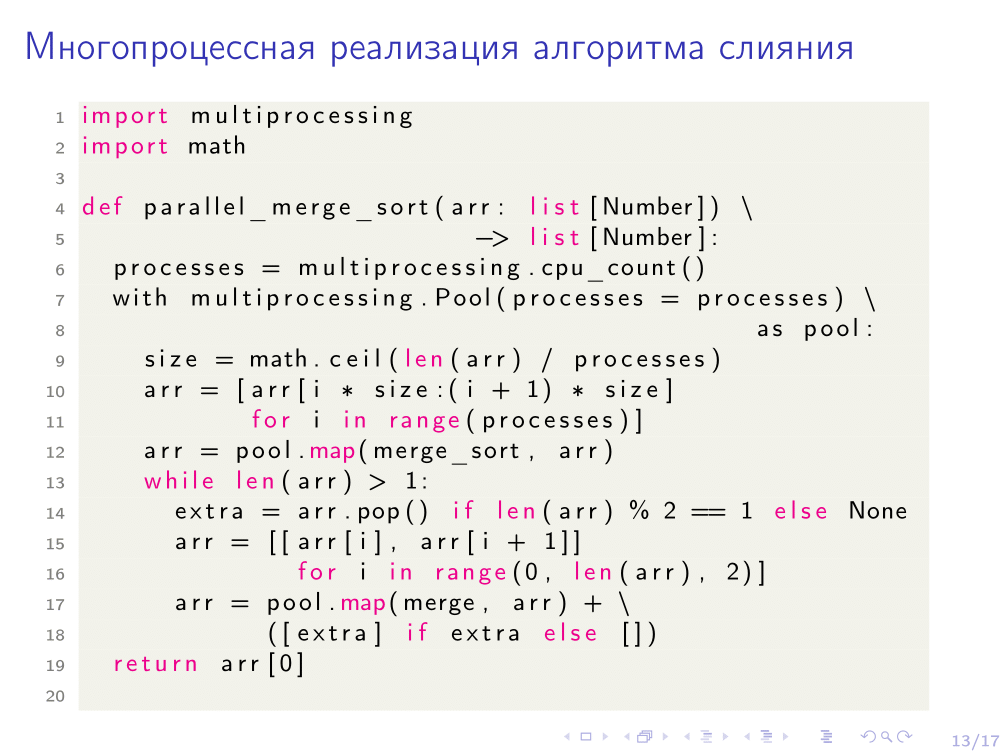
\includegraphics[scale=.7]{presentation-13.png}
	\end{figure}
	
	На слайде 14 представлена часть кода с 6 по 14 строку, на слайде 15 представлена часть кода с 13 по 19.
	
	\textit{Примечание:} Строка 7 на данном слайде является строкой 4 на слайде 14.
	
	\section{Слайд~14}
	\begin{figure}[H]
		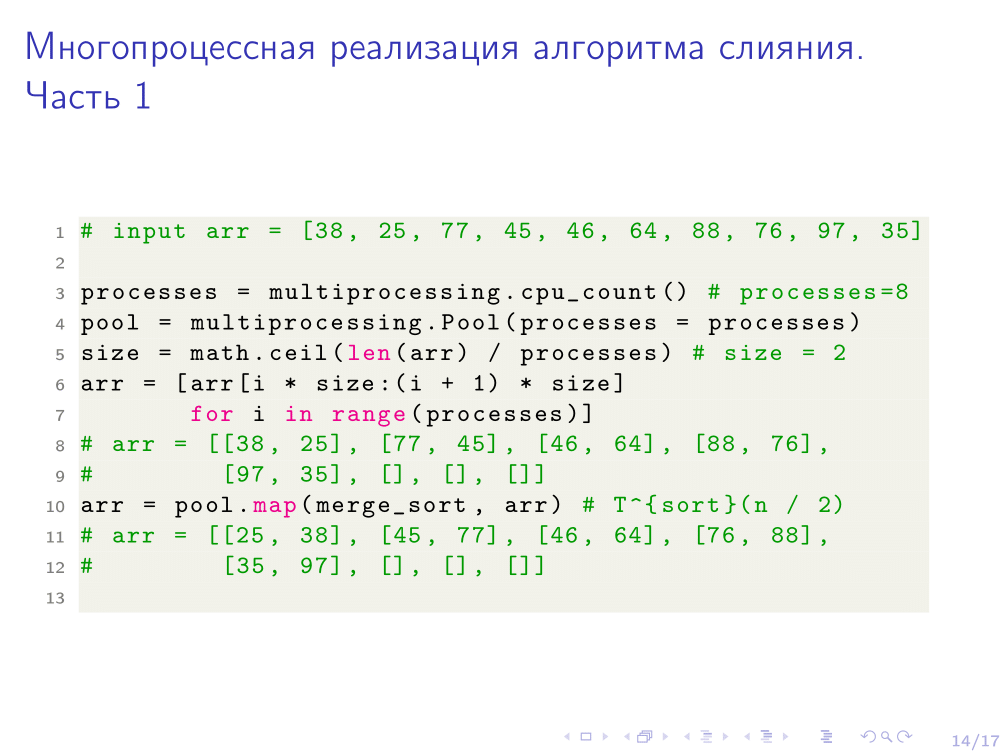
\includegraphics[scale=.7]{presentation-14.png}
	\end{figure}
	
	\begin{description}
		\item[1] Дан массив из 10 элементов;
		\item[3] Определение, сколько компьютер имеет ядер;
		\item[4] Создание бассейна процессов с размером, равным кол-ву ядер;
		\item[5] Определение, какого размера будут массивы, отданные процессам;
		\item[6--9] Разбиение исходного массива на массивы, количество которых равно кол-ву ядер;
		\item[10-12] Применение для каждого полученного после разбития массива функции \verb*|merge_sort| параллельно (в зависимости от размера бассейна \verb*|pool| доступных ядер). \verb*|arr| становится равен массиву с массивами с отсортированными элементами.
	\end{description}

	\section{Слайд~15}
	\begin{figure}[H]
		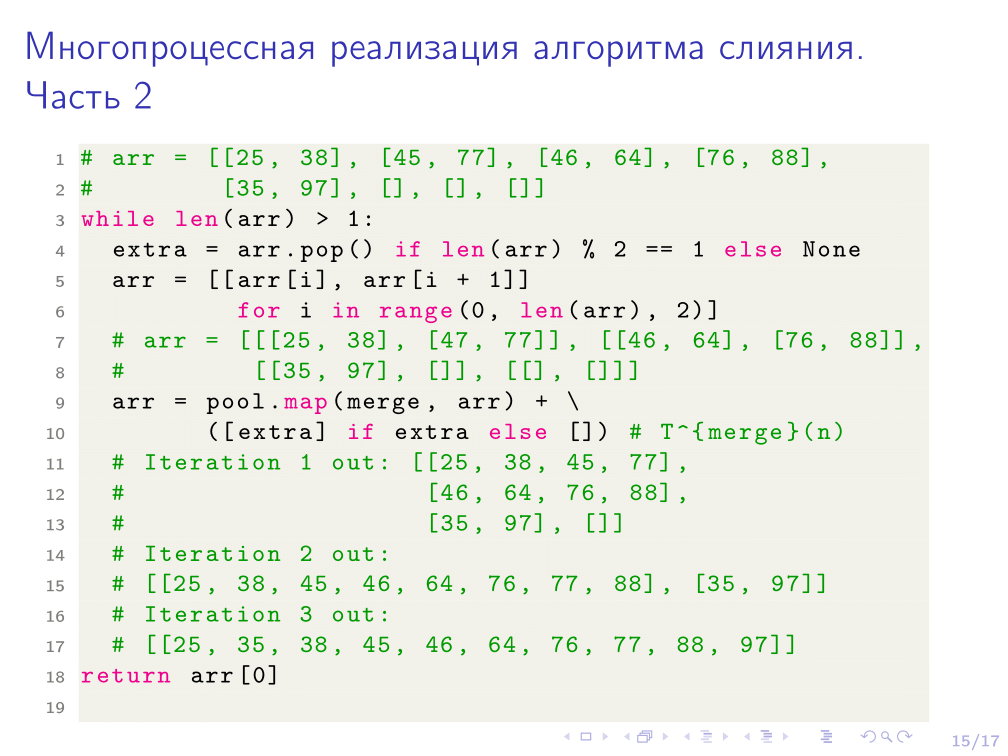
\includegraphics[scale=.7]{presentation-15.png}
	\end{figure}
	
	Отсортированные массивы необходимо слить.
	
	\begin{description}
		\item[3] Пока не остался один внутренний массив:
		\begin{description}
			\item[4] Если пары для последнего внутреннего массива не нашлось, то он будет \verb*|extra|;
			\item[5--8] Внутренние массивы объединить в пары;
			\item[9--13] Для каждой пары применить функцию \verb*|merge| и добавить \verb*|extra| массив с элементами;
		\end{description}
		\item[18] Вернуть слитый массив.
	\end{description}

	\section{Слайд~16}
	\begin{figure}[H]
		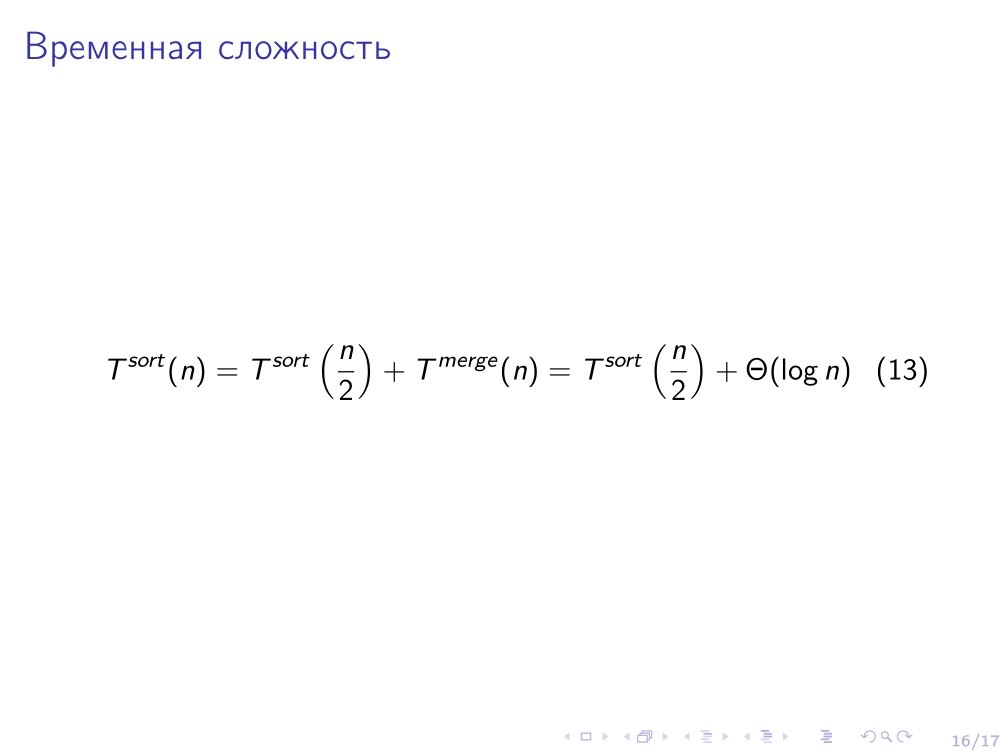
\includegraphics[scale=.7]{presentation-16.png}
	\end{figure}
	
	
\end{document}